\chapter{Scientific Background}
%labels will help you to reference to certain images, tables, chapters, section, and so on...
\label{background}

% DELETEME: This chapter will cover all of your background information and related work. Background and related work are directly related to your thesis. Please do not place irrelevant content here which is a common mistake. Citing will be handled in the appendices.

% DELETEME: Background represents underlying knowledge that is required to understand your work. The expected knowledge level of your readers can be set to the one of a bachelor or master student who just finished his studies (depending on what kind of thesis you are writing). This means that you do not need to describe how computers work, unless your thesis topic is about this. Everything that an average alumnus from your field of studies should know does not need to be described. It turns, background information that is very complex and content-wise very near to your problem, can be placed in the main parts. Everything else should be written here. Note: it is important to connect each presented topic to your thesis. E.g. if you present the ISO/OSI layer model you should also write that this is needed to understand the protocols you plan to develop in the main parts.

% DELETEME: Related work represents results from work that handled the same or a similar problem that you are addressing. This work might have used a different approach or might not have been that successful. Finding a paper / work that solved your problem in the same way you were planning to do is not good and you should contact your supervisor for solving this issue. Again, each paper / work has to be connected to your approach: other papers might have not chosen an optimal solution; they might not have been taking care of essential aspects; they might have chosen a different approach and you believe, yours will work better ...

This chapter introduces some important scientific fundamentals for better understanding of the problem's solution. Initially, \ref{camera_section} explains about the composition of a single digital pinhole camera and some of its characteristics. Then, \ref{camera_model} outlines the mathematical model for transforming a 3D object on the 2D image plane, after which the subsection \ref{instance_camera} informs about the functionality of the instance segmentation camera that CARLA offers. Finally, section \ref{carla_background} describes how the 3D autonomous driving simulator works and presents some of its features used in this work.

%###################################################################################
%###################### Topic A             ########################################
%###################################################################################
\section{Camera}\label{camera_section}
The digital camera is an instrument used for creating images through light capturing. On the figure \ref{fig:camera_construction} we could get an idea of how this technological invention is constructed. It uses an optic that consists of one or more lenses, through which the light rays are received. Afterwards, there is a sensor resembling the form of a solar panel, divided into red, green and blue pixels, which is hit by the collected light rays. As described from Schreer in \cite{camera_pinhole_model} the process of transforming the information from the captured light into a meaningful for the human eye representation is the following one: 
\begin{itemize}
    \item Light ray hits a sensor's pixel $\rightarrow$ The sensor converts it into an energy signal, which sends to the built-in computer $\rightarrow$ The computer estimates how dark or light the according pixel on the image plane should be and determines the correct colour value $\rightarrow$ As an output all pixels are combined in order to approximately recreate all details from the captured object  
\end{itemize}

In order to display a more detailed version of the captured image, cameras need more pixels to collect light rays\footnote{\url{https://www.creativelive.com/photography-guides/how-does-a-camera-work}, visited on 18/11/2022}. Thus, modern cameras rely on a bigger number of pixels to enhance the quality of the photos, which also contributes to improving the resolution of the visual sensor. Cameras with greater resolution are important in the area of street surveillance because in case of accidents or an against-the-rules behaviour it facilitates the task of recognising the suspect. Moreover, when we take into account the fact that these sensors act as a visual world perception for the autonomous vehicles, the resolution plays an essential role in the efficient object detection \cite{resolution_importance}. 

Another specification of cameras that this thesis considers is the so-called field of view (FoV), which determines the quantity of information that has been captured on the result image. It depends on the focal length of the lens and the sensor's size. On figure\footnote{\url{https://www.princetoninstruments.com/learn/camera-fundamentals/field-of-view-and-angular-field-of-view}, visited on 18/11/2022 \label{fov_figure}} \ref{fig:camera_fov} is shown what happens when the light goes through the lenses. In the upper case, due to a shorter focal length\footnote{The length between the lens and the focused image on the sensor} the lens converges the light stronger, therefore the focus is on the subject being imaged and the FoV is larger. In the vice-versa situation, the longer focal length allows for a focus on the image and thus provides a smaller FoV.

The monocular cameras belong to the directional sensors, because they can perceive information only from the direction in which their optical part is adjusted. In contrast to LiDAR sensors, which has a 360$^{\circ}$ view of the environment around it and can not be affected by light
conditions, single cameras are unreliable when exposed to bad light and weather conditions \cite{camera_vs_lidar}. As a main drawback of single cameras is regarded the lack of depth information, which impedes an accurate object recognition. Nevertheless, monocular cameras have advantages like lower integration price, much bigger availability on the market and the most important one is that they provide detailed pixel intensity information in form of a visual representation of the real world.
\begin{figure}
\centering
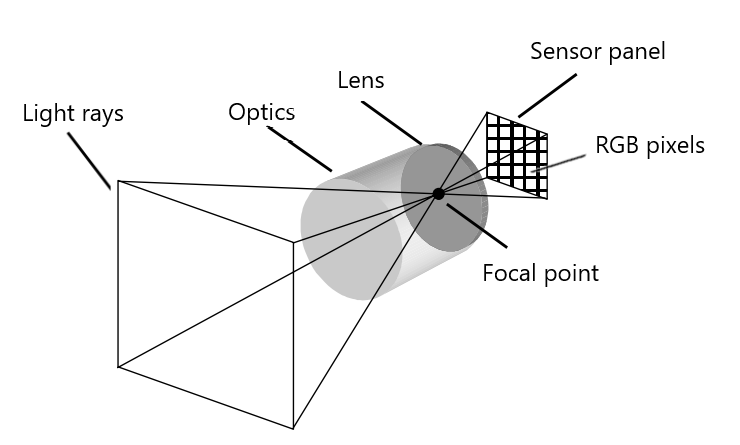
\includegraphics[width=0.8\textwidth]{images/camera_construction.png}
\caption[Digital camera's design]{This image illustrates simply the design of a digital camera, based on Schreer's book \cite{camera_pinhole_model} \label{fig:camera_construction}}
\end{figure}

\begin{figure}
\centering
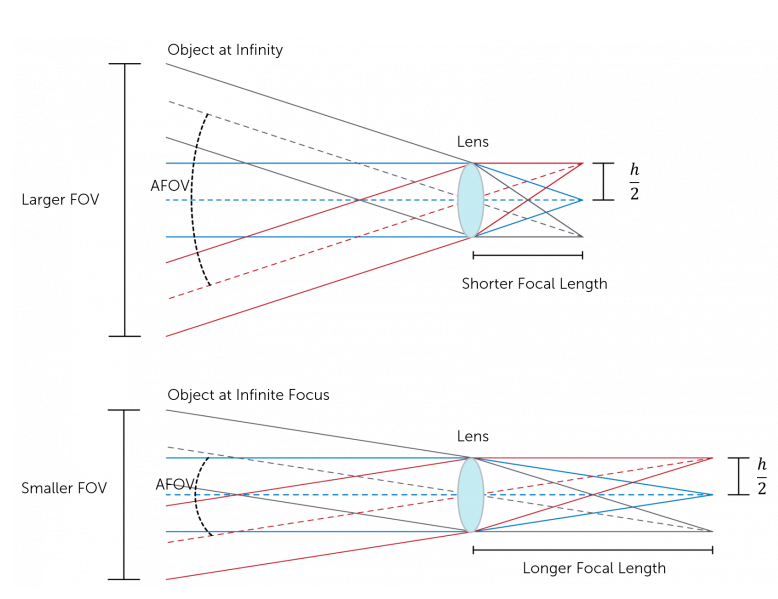
\includegraphics[width=0.8\textwidth]{images/camera_fov.png}
\caption[Single camera's FoV]{Depicting the influence of the focal length on the field of view, authored by footnote \ref{fov_figure} \label{fig:camera_fov}}
\end{figure}

\subsection{Camera model}\label{camera_model}
In order to illustrate how the transformation from a 3D world coordinate point to a 2D sensor's coordinate system happens, we use the pinhole camera model from Schreer \cite{camera_pinhole_model}. Figure TO\_BE\_ADDED portrays how a point $P$ from a real world object in front of the camera is orthogonally projected on the image plane. We then get the point $C$ definded in the image plane's coordinate system as $(u,v)^{T}$

\subsection{Instance Segmentation Camera}\label{instance_camera}

%###################################################################################
%###################### Topic B             ########################################
%###################################################################################
\section{CARLA - 3D autonomous driving simulator}\label{carla_background}

%###################################################################################
%###################### Topic C             ########################################
%###################################################################################
\section{Related Work}